\newpage
\section{RELATED THEORY}
\subsection{Architectural Explanations}
Image Super Resolution upscales a Low-Resolution Image to High Resolution Image, filling in the missing pixels with the different techniques. There are other simpler methods to upscale images like Linear or Bi-cubic interpolation, but they do not generate any new information based on the environment and hence are not super useful to upscale an LR image. Deep Learning based methods require huge amounts of data so that the model is not overfitted, the dataset needs to contain an HR and LR version of the same image that are perfectly aligned to each other. We need to synthetically create LR images from HR images.\\
SR aims to then reverse whichever degradation process is considered, to retrieve the original underlying high-fidelity image. We have implemented SRCNN, SSResNet and SRGAN. Their architecture is explained below: 
\begin{enumerate}[label=(\roman*)]
    \item {\bf SRCNN:} Super-Resolution Convolutional Neural Network, is a deep learning architecture devised for single-image super-resolution tasks. Developed by {\bf Dong et al. in 2014} \cite{r2}, SRCNN revolutionized image enhancement by learning complex mappings between low-resolution and high-resolution images directly from data. Its architecture consists of multiple layers of convolutional neural networks (CNNs), which process input images in a hierarchical manner, gradually extracting high-level features. The architecture of SRCNN is given below:
    \begin{figure}[ht]
        \centering
        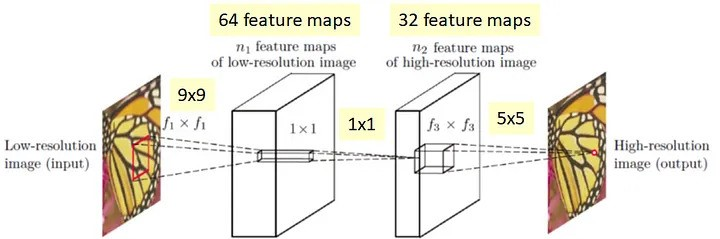
\includegraphics[width=5in]{./figures/srcnn.jpg}
        \caption{SRCNN Architecture}
        \par  Source: \url{https://arxiv.org/pdf/1501.00092}
    \end{figure} \\
    We converted image from training database into Y,Cb,Cr format and used only Y (Luminance) component for training the model. The primary loss function used in SRCNN is Mean Squared Error (MSE). We used Adam optimizer, optimizer is responsible for updating the network's parameters during the training process in order to minimize the chosen loss function.

    \item {\bf SRResNet:} The SRResNet is a fully convolutional network designed for 4x super-resolution. It incorporates residual blocks with skip connections to increase the optimizability of the network despite its significant depth. The SRResNet is trained and used as a standalone network and provides a nice baseline for the SRGAN – for both comparison and initialization. We use the following architecture for this network. 
    \begin{figure}[ht]
        \centering
        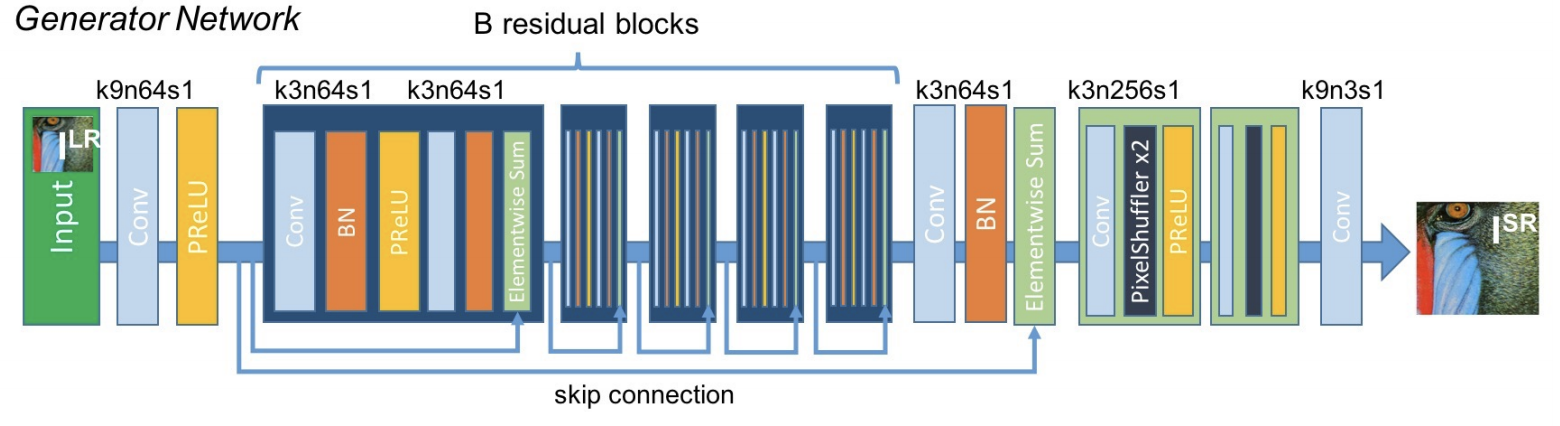
\includegraphics[width=6in]{./figures/generator.png}
        \caption{SRResNet Architecture or Generator of SRGAN}
        \par  Source: \url{https://arxiv.org/pdf/1609.04802}
    \end{figure} \\
    The SRResNet first contains convolution block of large Kernel Size 9x9, stride of 1 and 64 channels with PreLU activation. There are 16 residual blocks with convolution layer of Kernel size 3x3 followed by batch normalization, PreLU same conv layer again and batch normalization again. The output then is passed through same 3x3 conv layer and batch normalized. Two subpixel convolution blocks are used followed by PreLU activation each of which provides two times upscaling. Finally, a convolution with large kernel size of 9x9 and 1 stride with 3 out channels for RGB is done with Tanh activation to get super resolved image.\\ In Forward Pass, SRResNet produces a 4x upscaled image from provided low-res image using the above architecture. Mean-Squared Error (MSE) is used as the loss function to compare the upscaled image and original high-quality image. MSE is a type of content loss but here it only looks in RGB space of predicted and target images. Minimizing the MSE by changing the parameters of the network will make the model produce images closer to the original images.
    
    \item {\bf SRGAN:} Super-Resolution Generative Adversarial Network consist of two adversary networks Generator and Discriminator which are trained in tandem. The goal of the Generator is to learn to super-sample an image such that Discriminator can’t tell difference between artificial and natural origins. The interplay between these two networks leads to the improvement of both over time. \\
    The Generator learns not only by minimizing content loss, as in the case of the SRResNet but also by spying on the Discriminator's methods. By providing the Generator access to the Discriminator's inner workings in the form of the gradients produced therein when backpropagating from its outputs, the Generator can adjust its parameters in a way that alters the Discriminator's outputs in its favour. As the Generator produces more realistic high-resolution images, we use these to train the Discriminator, improving its discriminating abilities.
    \begin{figure}[ht]
        \centering
        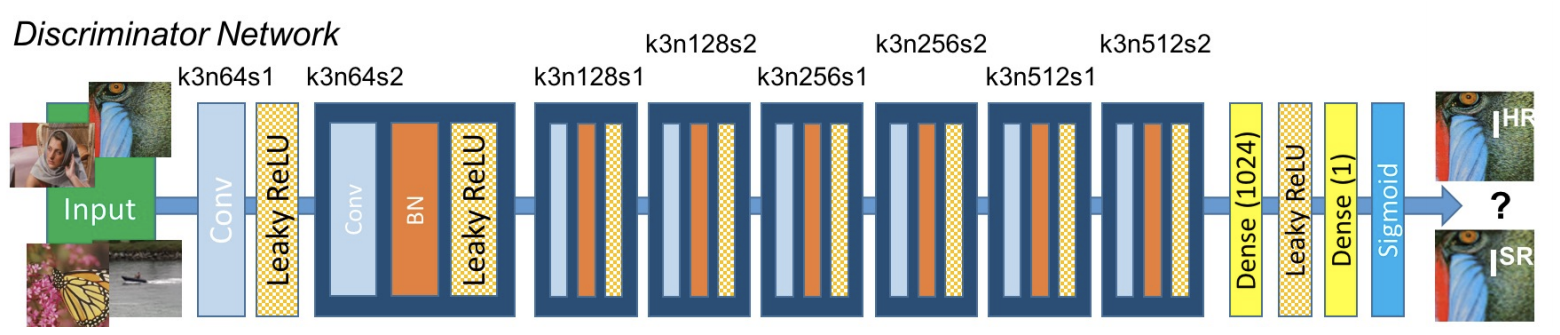
\includegraphics[width=6in]{./figures/discriminator.png}
        \caption{Discriminator Architecture}
        \par  Source: \url{https://arxiv.org/pdf/1609.04802}
    \end{figure} \\
    The Generator has same architecture as SRResNet. Training Discriminator is not different from any binary image classifier. It is trained on both real images and generated images from generator. In Forward Pass, it outputs the probability score $P_{HR}$. If the provided image was real, we desire the $P_{HR}$ to be as high as possible towards 1. And for generated image as low as possible towards 0. We use Binary Cross Entropy loss $-logP_{HR}$ when input image is real and $-logP_{SR}$ when image is generated. Here $P_{SR}=1-P_{HR}$. Minimizing these losses by changing the parameters will make discriminator predict higher probability for real images and lower probability for generated images.\\
    We use better content loss than that of SRResNet. In ResNet we use MSE loss in RGB space which produces overly smooth images with no finer details. There are a lot of possibilities of similar pixel combination that can be formed from low resolution image patch. When we use content loss in RGB space, it averages the output rather than choosing one of the combinations which would produce better result as an overly smooth “averaged” prediction will always have lower MSE.\\
    We can use CNN trained to classify images to find deeper meaning of patterns in images. This new representation space is more suitable for calculating content loss and can hallucinate new details showing creativity. We specifically use the VGG19 network as recommended in the paper. We use MSE-based content loss in this VGG space to compare the images. The use of content loss is only one component of the generator update, we use adversarial loss obviously. The super-resolved image is passed through the Discriminator with its weight frozen not to update the discriminator but to get the probability score $P_{HR}$ with misleading label and use the BCE loss $-logP_{HR}$ and resulting gradient information to update the Generator’s weights such that it produces images closer to its natural origin.
    GAN is trained in an interleaved fashion, where the generator and discriminator are alternatively trained for short periods of time just once before making the switch in this case.
\end{enumerate}
    \subsection{General Explanations}
    \begin{enumerate}[label=(\roman*)]
        \item {\bf Conv2d:} Conv2D stands for two-dimensional convolution, a fundamental operation in convolutional neural networks (CNNs). A convolutional layer applies a series of filters or kernels to an input image. Each filter detects specific patterns or features, like edges, textures, or shapes. The convolution operation involves sliding these filters over the input image, performing element-wise multiplication between the filter and the overlapping portions of the image, and then summing up the results to create a feature map.
        \begin{figure}[ht]
            \centering
            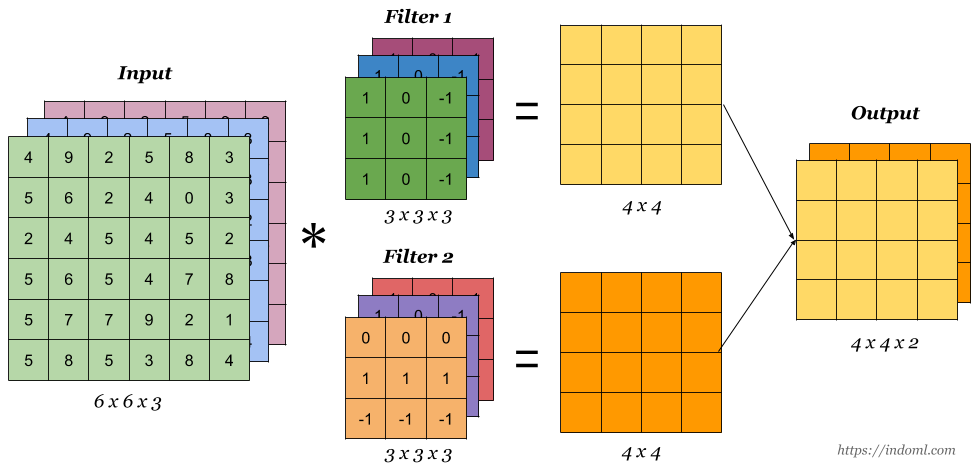
\includegraphics[width=5in]{./figures/conv2d.png}
            \caption{A visual explanation of convolution. }
            \par  Source: \url{https://indoml.files.wordpress.com/2018/03/convolution-with-multiple-filters2.png}
        \end{figure} \\
        \begin{itemize}
            \item {\bf Kernel:} A kernel describes a filter that we are going to pass over an input image. The kernel will move over the whole image, from left to right, from top to bottom by applying a convolutional product. The output of this operation is called a filtered image.
            \item {\bf Stride:} Stride refers to the number of steps the convolutional filter moves horizontally or vertically during convolutional operation. For example, a stride of 2 means the filter moves two pixels at a time.
            \item {\bf Padding:} Padding describes the number of pixels added to the sides of the input channels before their convolutional filtering. Usually padding pixels are set to zero. This is particularly useful when we want the size of the output channels to be equal to the size of the input channels. When the kernel size is  3*3  then the output channel size is decreased by one on each size. To overcome this problem, we can use padding of 1.
            \item {\bf In channel:} In channel are used to describe how many channels are present in the input. For instance, if the input is an RGB image, then it has three channels. When using a Conv2d layer, we can specify the number of in channel, and the convolution operation is performed independently on each channel of the input. This allows the network to learn different features from different input channels, enabling it to detect various patterns within each channel.
            \item {\bf Out Channel:} Out Channel specifies the number of output channels produced by the convolutional layer. Each output channel corresponds to a distinct convolutional filter (or kernel) applied to the input.
        \end{itemize}
        \item {\bf Batch Normalization:} Batch normalization is a technique that normalizes the inputs to each layer in a network by adjusting and scaling to have zero mean and unit variance. This helps to reduce “internal covariate shift” problem which can hinder training. An internal covariant shift occurs when there is a change in input distribution to the network. When the input distribution changes, hidden layers try to learn to adapt to the new distribution. This slows down the training process. If a process slows down, it takes a long time to converge to a global minimum. Batch normalization transform the data so that its values have similar scale, making it easier for the network to learn and converge faster. \par
        Formula for batch normalization:      
        \begin{equation}
        y = \frac{x - E [x]}{\sqrt{Var[x] + \epsilon }}+\gamma + \beta    
        \end{equation}      
         
        where, $\beta$ and $\gamma$ are learnable parameter vector. \\ 
        X represent the value of the feature map/channel.\\
        Var[X] is the variance of the mini batch for the feature map/channel.\\
        $\epsilon$ is small constant.\\
        \item {\bf Activation Function:} Activation function decides whether a neuron should be activated or not. This means that it will decide whether the neuron’s input to the network is important or not in the process of prediction. The primary role of the activation function is to transform the summed weighted input from the node into an output value to be fed to the next hidden layer or as output. Different types of activation function used in our project is listed below:
        \begin{itemize}
            \item {\bf Tanh:} Tanh function is similar to the sigmoid activation function, and even has the S-shaped with the difference in output range of -1 to 1. In Tanh, the larger the input (more positive), the closer the output value will be to 1.0, whereas the smaller the input (more negative), the closer the output will be to -1.0. 
            \begin{figure}[ht]
                \centering
                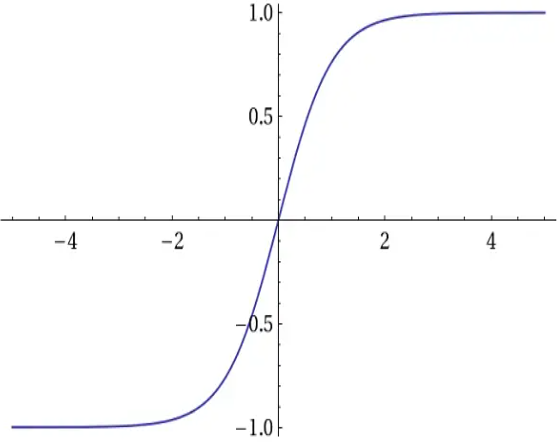
\includegraphics[width=2.2in]{./figures/tanhcurve.png}
                \caption{ Tanh curve}
            \end{figure} \\
            \item {\bf ReLU:} ReLU stands for Rectified Linear Unit. Although it gives an impression of a linear function, ReLU has a derivative function and allows for backpropagation while simultaneously making it computationally efficient. The main catch is that ReLU function does not activate all the neurons at the same time. The neurons will only be deactivated if the input to the ReLU function is less than zero. \cite{r6}
            \begin{figure}[ht]
                \centering
                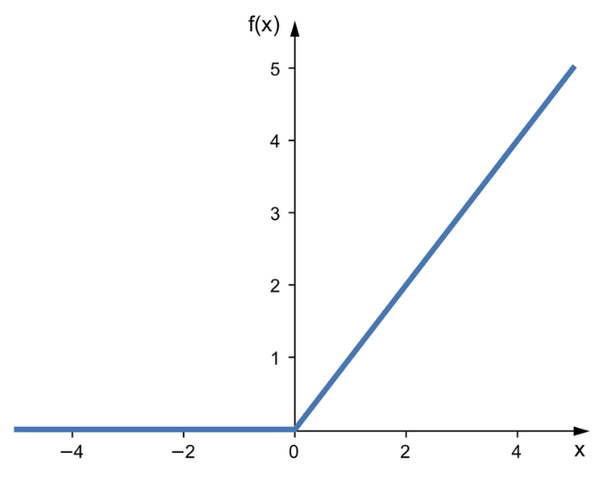
\includegraphics[width=2.5in]{./figures/relucurve.png}
                \caption{ Relu curve}
            \end{figure} \\
            Mathematically it can be represented as:
            \begin{equation}
                R(x) =\left \{\frac{x}{0} \ \ \ \ \begin{matrix}
                    if \ x\geq 0 & \\ if \ x < 0
                    & 
                   \end{matrix} \right\}
            \end{equation}
               The major limitation of ReLU is Dying ReLU problem. The negative side of the graph makes the gradient value zero. Due to this reason, during the backpropagation process, the weights and biases for some neurons are not updated. This can create dead neuron which never get activated.
            \item {\bf Leaky Relu:} : Leaky ReLU is an improved version of ReLU function to solve the Dying ReLU  problem as it has small positive slope in the negative area. The advantage of Leaky ReLU is same as ReLU, in addition to the fact that it does enable backpropagation, even for negative input values. By making this minor modification for negative input values, the gradient of the left side of the graph comes out to be a non-zero value.\\
            The limitation faced by Leaky ReLU is the prediction may not be consistent for negative input values.\\
            Mathematically it can be represented as:
            \begin{equation}
                f(x) =\left \{\frac{x}{0} \ \ \ \ \begin{matrix}
                    if \ x\geq 0 & \\ if \ \alpha * x < 0
                    & 
                   \end{matrix} \right\}    
            \end{equation}
            
            \begin{figure}[ht]
                \centering
                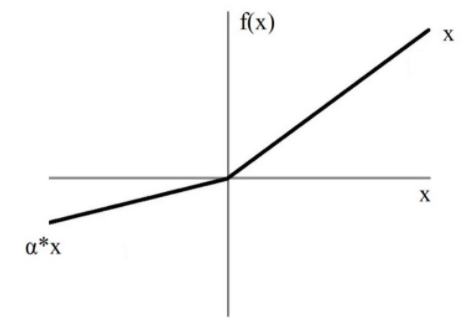
\includegraphics[width=2.6in]{./figures/leakyrelucurve.png}
                \caption{Leaky Relu curve}
            \end{figure}
            \item {\bf Prelu:}Parametric ReLU is another variant of ReLU that aims to solve the problem of gradient’s becoming zero for the left half axis. This function provides the slope of the negative part of the function as an argument.\cite{r5}
            \begin{figure}[ht]
                \centering
                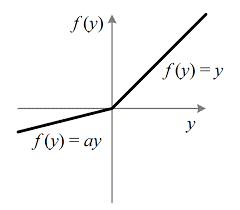
\includegraphics[width=2.5in]{./figures/prelucurve.png}
                \caption{Parametric Relu curve}
            \end{figure} \\
            Mathematically it can be represented as:
            \begin{equation}
                R(x) =\left \{\frac{x}{0} \ \ \ \ \begin{matrix}
                    if \ x\geq 0 & \\ if \ a * x < 0
                    & 
                   \end{matrix} \right\} 
            \end{equation}
           
               where ‘a’ is the slope parameter for negative values. Prelu can learn slope parameter using backpropagation at a negligible increase in the cost of training.
        \end{itemize}
        \item {\bf Pixel Shuffle:} The Pixel shuffle is a technique used in image super resolution to upscale an image by a factor of r. It works by rearranging the pixels in a feature map of size $(W,H,C * r^2)$ to form a super-pixel feature map of size (r*W, r*H, C). \cite{r7}\\The pixel shuffle operation can be described as follows:
        \begin{itemize}
            \item For each pixel in the input feature map, split its value into $r^2$ sub-pixels.
            \item Arrange the sub-pixels in grid-like pattern, with each sub-pixels occupying a position in a feature map.
        \end{itemize}
        \begin{figure}[ht]
            \centering
            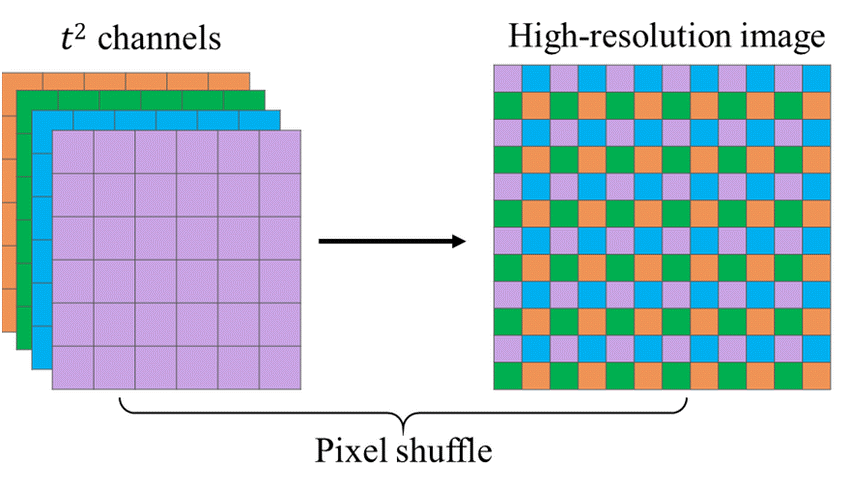
\includegraphics[width=3in]{./figures/pixelshuffle.png}
            \caption{Pixel Shuffle}
            \par  Source: \url{https://production-media.paperswithcode.com/methods/pixelshuffle_Ed27NA5.pbm}
        \end{figure}
        \item {\bf Residual Block:} A residual block is a building block that contains one or more convolutional layers and a skip connection. The skip connection allows gradient to flow through the network more efficiently, improving the training process and avoiding the vanishing gradient problem.
        \begin{figure}[h!]
            \centering
            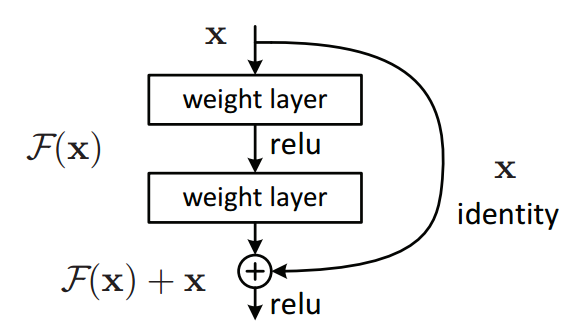
\includegraphics[width=3in]{./figures/residualblock.png}
            \caption{Residual block}
        \end{figure}
    \end{enumerate}
    \nocite{r8}
